\begin{frame}[fragile]
    \frametitle{C\'omo crear un branch?}
    ¿y qu\'e es un branch?. La traducci\'on literal ser\'ia: rama.
    Es decir, dentro de nuestro sistema de control de versiones podemos ver
    el hist\'orico de cambios como si de un \'arbol se tratase. 
    De esta forma podemos ir abriendo ramas que parten bien de la rama 
    principal (master) o de otra rama (branch).
    \begin{figure}
        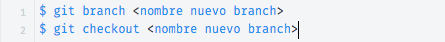
\includegraphics[width=1\textwidth]{Images/13.png}
    \end{figure}
    Con esto creamos un branch y con el checkout nos movemos a \'el 
    (el working directory queda apuntando a este branch para poder trabajar 
     con el).
\end{frame}

\begin{frame}[fragile]
    \frametitle{Visualiar los Branch que tenemos}
    Ejecutamos el comandos \alert{git branch} y obtendremos una salida de 
    este estilo:
    \begin{figure}
        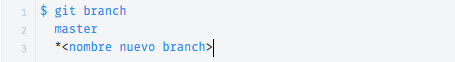
\includegraphics[width=1\textwidth]{Images/14.png}
    \end{figure}
    Donde el \'* indica el branch activo. El listado anterior solo muestra 
    los branch locales, pero tambi\'en podemos listar los branch remotos si 
    hacemos: \alert{git branch -a}.
\end{frame}
